\documentclass[a4paper,11pt]{jsarticle}
\usepackage{amsthm} %定理系を入れるのに必須
\usepackage{amsmath,amssymb} %\dfrac
\usepackage{bm} %\bm:斜体太字の文字を書けるようにする(ベクトル表記)
\usepackage{ascmac} %参考http://akita-nct.jp/yamamoto/comp/latex/make_doc/box/box.php
\usepackage{fancyhdr} %ヘッダに任意の文字列を書く
\usepackage{amsfonts} %\mathbb:白抜き文字を書けるようにする
\usepackage{enumerate}
\usepackage[english]{babel}

\usepackage[dvipdfmx]{graphicx} %図表を入れる場合
\usepackage{float} %図表の位置
\usepackage{subfigure}



\makeatletter
   \renewcommand{\theequation}{%
   \thesection.\arabic{equation}}
   \@addtoreset{equation}{section}
\makeatother

\theoremstyle{definition}
\newtheorem{theorem}{Thm.}[subsection] 
\newtheorem{definition}{Def.}[subsection]
\newtheorem{lem}{Lem.}[subsection]
\newtheorem{prf}{Prf.}[subsection]
\newtheorem{prop}{Prop.}[subsection]
\newtheorem{ex}{Ex.}[subsection]
\newtheorem{asm}{Asm.}[subsection]

%ナンバリングを外したいとき
\newtheorem*{theorem*}{Thm.} 
\newtheorem*{definition*}{Def.}



%偏微分,チルダ,分数
\newcommand{\pd}[2]{\dfrac{\partial #1}{\partial #2}}
\newcommand{\pdd}[2]{\dfrac{{\partial}^2 #1} {\partial {#2}^2} }
\newcommand{\ti}[1]{\tilde{#1}}
\newcommand{\df}[2]{\dfrac{#1}{#2}}
\newcommand{\intinf}{\int_{-\infty}^{\infty}}

\title{Advanced Derivative}
\author{Kohei Fukushima}
\date{\today}

\begin{document}
\maketitle
\pagestyle{fancy}
\lhead{Kohei Fukushima}
%\rhead{\today}
\rhead{\rightmark}

% \newpage
% \thispagestyle{empty}
% \tableofcontents %目次

\section{Bond and Forward Contract}
\subsection{Interest Rates}
\begin{asm}
  We asssume that there exists a default free
  money market account
  \begin{itemize}
    \item default-free
    \item liquid (borrowing ragte = lending rate)
    \item everyone can access equally
  \end{itemize}
\end{asm}

The interest rates associating with the default free m.m.
(money market) are called risk-free rates.


\subsubsection{Types of Accrual (利息)}
Suppose one invests cash amount $A$ at $t=0$ for $T$ years. \\
$V$ : The amount of cash to be returned in $T$ years time.

\begin{enumerate}
  \item Annual compounding with interest rate $R_1$ per annum\\
  $V=A(1+R_1)^T$
  \item Semiannual compounding with interest rate $R_2$ per annum\\
  $V=A(1+\frac{R_2}{2})^{2T}$
  \item m-times compounding with interest rate $R_m$ per annum\\
  $V=A(1+\frac{R_m}{m})^{mT}$
  \quad (typiccaly we have $m=1,2,4,12,52,365$)
  \item continuous compounding with interest rate $r$ per annum\\
  $V=\lim_{m\to\infty}A(1+\frac{r}{m})^{mT}=Ae^{rT}$  
\end{enumerate}

Relation among different compounding conventions:

\underline{No-Arbitrage}
\quad $\to$ for any $m$, 
\begin{align}
  e^{rT}&=\left(1+\df{R_m}{m}\right)^{mT} \\
  \Leftrightarrow \quad r&=m \ln\left(1+\df{R_m}{m}\right),
  \quad R_m=m(e^{r/m}-1).
\end{align}

at a given time, $R_1(T)$ : $T$ dependent. 


\subsubsection{Zero Rate and Bonds}
%https://ja.sharelatex.com/learn/Theorems_and_proofs
%http://iso.2022.jp/math/abbrev/
\begin{definition}{(zero rate)}
The T-year zero-coupon interest rate is the rate of interest 
earned on an investment that starts today and lasts for T-years
without any intermidiate coupon payment.
\end{definition}

\begin{ex}
  5-year zero rate = 5 \% per annum. (continuous compounding)\\
  \$ $100$をdeposit at $t=0$ $\to$ (5 years later) 
  $100e^{0.05\times 5} \approx 128.40 $
\end{ex}

Present value (PV) \quad
$P.V.=128.40 \times e^{-0.05\times 5} = 100 $

\begin{definition}{(ZCB : zero coupon bond)}
  T-year zero coupon bond is a bond which pays an unit amount
  of cash in T-year time without any coupon payment
  (assume risk-free, liquid).
\end{definition}

If $R$ is T-year zero rate, 
current price of T-year zero coupon Bond is given by :
\begin{align}
  P(0,T)=e^{-RT}
\end{align}
($0$: current time, $T$: maturity), \quad
we call "discount factor".

\begin{ex}\label{bondprice}
  Suppose we have (at $t=0$)
  \begin{itemize}
    \item $T=0.5, \, R=5.0\%$ \, (zero coupon rate)
    \item $T=1.0, \, R=5.8\%$
    \item $T=1.5, \, R=6.4\%$
    \item $T=2.0, \, R=6.8\%$
  \end{itemize}
  fixed coupon bond
  \begin{itemize}
    \item maturity: $T=2$
    \item coupon payments: 6\% per annum semiannually.
    \item principal: \$100
  \end{itemize}
  \begin{align}
    \mbox{Bond price}&=3P(0,0.5)+3P(0,1.0)+3P(0,1.5)+103P(0,2) \notag\\
    &=3\times e^{-5\%\times 0.5}+3\times e^{-5.8\%\times 1.0}
    +3\times e^{-6,4\%\times 1.5}+103\times e^{-6.8\%\times 2.0} \notag\\
    &\approx 98.39
  \end{align}
\end{ex} 


\subsubsection{Yield (平均利率,平均利回り,平均discount rate)}
\begin{definition}{(Bond's Yield)}
  A bond's yield is the single discount rate
  that when applied to eery cash flow,
  gives the market bond price.
\end{definition}

\begin{ex}
  using Ex. \ref{bondprice}, 
  suppose $\mbox{market price} = 98.39$ \\
  Then the yield for the bond $y$ is given by solving
  \begin{align}
    &3e^{-0.5y}+3e^{-1.0y}+3e^{-1.5y}+103e^{-2.0y} = 98.39 \\
    \Rightarrow& y \simeq 6.76\% \quad \mbox{(continuous compounding)}
  \end{align}
\end{ex}

\begin{definition}{(Par Yield)}
  The par yield for a certain maturity is the coupon rate
  that makes the bond price equal to its principal.
\end{definition}

\begin{ex}
  using Ex. \ref{bondprice}, 
  par yield $C$ for 2-year coupon bond is given by:
  \begin{align}
    &\df{C}{2}e^{-0.050\cdot 0.5}+\df{C}{2}e^{-0.058\cdot 1.0}
    +\df{C}{2}e^{-0.064\cdot 1.5}
    +\left(100+\df{C}{2}\right)e^{-0.068\cdot 2.0}=100 \\
    \Rightarrow& C\simeq 6.87\%
  \end{align}
  (par yield for $T=2$, semiannual coupon payments) \par
  In general, 
  \begin{itemize}
    \item T-year bond
    \item m-time coupon payment per annum
    \item par yield $C$
  \end{itemize}
  \begin{align}
    &\sum_{n=1}^{mT}\df{C}{m}P\left(0,\df{n}{m}\right)+100P(0,T)=100 \\
    \Rightarrow& C=\df{100(1-P(0,T))}{A}, \quad
    A=\sum_{n=1}^{mT}\df{1}{m}P\left(0,\df{n}{m}\right)
  \end{align}
\end{ex}


\subsubsection{Duration}
fixed coupond bond:
\begin{itemize}
  \item $(\mbox{cash flow at } T_i) =C_i \quad (i=1, ..., n)$
  \item $C_i$: coupon (+ principal at maturity)
\end{itemize}
Suppose its yield is given by $y$ (continuous compounding).\\
Bond price: 
\begin{align}
  B=\sum_{i=1}^{n}C_i e^{-yT_i}
\end{align}
The duration of the Bond:
\begin{align}
  D:=-\df{1}{B} \df{d}{dy} B= -\left(\df{dB/dy}{B} \right) 
  =\df{1}{B}\sum_{i=1}^{n}C_i T_i e^{-yT_i}
\end{align}

\begin{ex}{zero coupon Bond}
  \begin{align}
    &(C_i=0)_{i=1,2,...,n-1}, \, C_n=1, \quad B=e^{-yT_n}\\
    \Rightarrow& D=\df{1}{B}C_n T_n e^{-yT_n}=T_n
  \end{align}
\end{ex}

(* Durationの長短により,金利に対する反応度の違いがわかる.)

Suppose the yield changes small amount $\Delta y$, 
($y\to y+\Delta y, \quad B\to B+\Delta B$) \\
\begin{align}
  \df{\Delta B}{B}=-D\Delta y + o(\Delta y)
\end{align}
(abbr.)

Suppose $D=10$ (10 year),
yield: $\Delta y=+0.1\%$ (10 basis points, b.p.):
\begin{align}
  \df{\Delta B}{B} \approx -10 \times 0.1\% =-1\%=-0.01
\end{align}


\subsubsection{Modified Duration}
yield (m-time compounding) $\hat{y}$ \\
the same bond: 
\begin{align}
  B=\sum_{i=1}^{n}C_i \left(1+\df{\hat{y}}{m}\right)^{-mT_i}  
\end{align}
modified duration:
\begin{align}
  D^{*}:&=-\df{1}{B} \df{dB}{d\hat{y}}
  =\df{1}{B}\sum_{i=1}^{n}\df{C_i T_i}{1+\hat{y}/m}
  \left(1+\df{\hat{y}}{m}\right)^{-mT_i} \notag\\
  &=\df{1}{B(1+\hat{y}/m)}\sum_{i=1}^{n}C_i T_i
  \left(1+\df{\hat{y}}{m}\right)^{-mT_i} \notag\\
  &=\df{1}{B(1+\hat{y}/m)}\sum_{i=1}^{n}C_i T_i e^{-yT_i}
  =\df{D}{1+\hat{y}/m} \quad (\mbox{no arbitrage})
\end{align}
* durationの議論はcash flowが一方向のときのみ使える.
Insuranceでは通用しないので注意.


\subsubsection{Convecity)}
$y$ : yiled (continuous compounding)
\begin{align}
  C:=\df{1}{B}\df{d^2B}{dy^2}
  =\df{1}{B}\sum_{i=1}^{n}C_i T_i^2 e^{-yT_i}
\end{align}
$y\to y+\Delta y, \quad B\to B+\Delta B$:
\begin{align}
  &\Delta B=\df{dB}{dy}\Delta y
  +\df{1}{2}\df{d^2B}{dy^2}(\Delta y)^2+o(\Delta y^2) \\
  \Rightarrow&\df{\Delta B}{B}=-D\Delta y
  +\df{1}{2}C(\Delta y)^2+o(\Delta y^2) 
\end{align}

(Duration matching : abbr.)



\subsection{Forward Contract}
\subsubsection{Forward Price}

\begin{definition}{(Forward Contract)}
  A forward contract with maturity $T$ is a bilateral binding
  promise(agreement) such that at time $t=T(>0)$,
  the two parties exchange:
  \begin{itemize}
    \item the cash amount given by the time $T$ realization of
    a certain index (such as a stock price) with the fixed amount of
    cash (cash delivery)
    \item the unit amount of asset (such as a share of an equity)
    with fixed amount of cash (physical delivery=現物)
  \end{itemize}
\end{definition}

\begin{definition}{(Forward Price)}
  A forward price $F$ at the current time ($t=0$) (契約時) of
  the underlying index $X$ is the amount of cash $K$ that make
  the present value of the forward contract exchanging $X_t$
  and $K$ at $T$ zero. 
  (Forward contract has $P.V.=0$, with $K=F$.)\\
  * $F$は契約時に支払う額ではないことに注意(元手は不要) \\
  * $K$ such that P.V. of the fwd contract $=0$
\end{definition}

\begin{ex}\label{fwd1}
  Consider a forward contract on a non-dividend paying stock,
  with mat. $T$.
  
  $X_T=S_T$ (stock price at $T$),
  exchange $F \leftrightarrow S_T$ (at $T$).
  \begin{asm}
    Stock market is liquid, zero-coupon bond is liquid.
  \end{asm}
  the forward price at $t=0$ is given by:
  \begin{align}
    F=\df{S_0}{P(0,T)}=e^{rT}S_0
  \end{align}
  \begin{itemize}
    \item $r$ : zero-rate for mat $T$, continuous, compounding
    \item $P(0,T)$ : zero coupon bond price
  \end{itemize}
  
  \begin{prf}{replication strategy}
    \begin{itemize}
      \item Enter the fwd contract to get one share of stock
      ($S_T$) by paying $F$ at $T$
      ($t=0$でenterする際に元手は不要)
      \item Sell one share of stock at $t=0$ to get $S_0$
      (short position)
      \item Use $S_0$ to buy ZCB (zero coupon bond) by the amount
      $S_0/P(0,T)$
      \item Pay $F$ and receive $S_T$ at $T$ (return $S_T$ to lender)
      \item Receive $S_0/P(0,T)$ from ZCB lender
    \end{itemize}
    (cash flow illustration below) \\
    if $F\neq \df{S_0}{P(0,T)} \Rightarrow$ arbitrage
    (no risk, arbitrary positive return) \\
    No-arbitrage $\Rightarrow F=\df{S_0}{P(0,T)}=e^{rT}S_0$
    ($F$はstochasticではない)
  \end{prf}
\end{ex}

\begin{figure}[H] %HはHereを意味する
  \begin{center}
    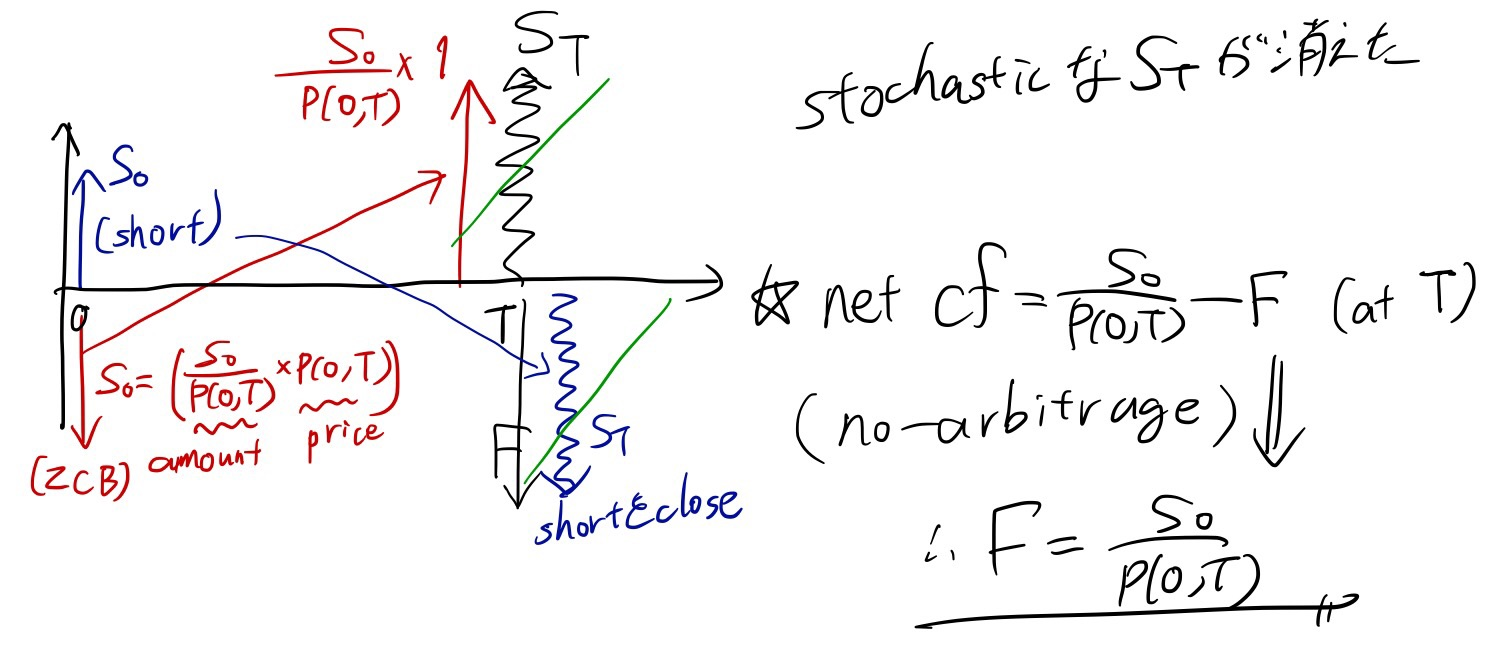
\includegraphics[width=10cm]{fig/1_2_01.JPG}
  \end{center}
\end{figure}

\begin{ex}
  Same as Ex.\ref{fwd1} but now the stock pays 
  \underline{continuous dividend}, with dividend rate $y$
  ($y\in \mathbb{R}$, constant)

  One share of the stock pays $S_t ydt$ for the interval
  $[t, t+dt]$ for any $t\geq 0$. \\
  \underline{forward price at $t=0$}
  \begin{align}
    F=\df{S_0}{P(0,T)}e^{-yT}=S_0 e^{(r-y)T}
  \end{align}
  $r$ : zero-rate for mat $T$ at $t=0$

  Suppose we heve $N_t$ shares at $t$,
  dividend paid in $[t, t+dt]: \, S_t N_t ydt$ \\
  $\Rightarrow$ reinvest $\Delta N_t = N_t ydt$

  if one reinvests the whole dividend payment, 
  \begin{align}
    \df{dN_t}{dt}=N_t y \, \Rightarrow \,
    N_t=N_0e^{yt} \quad \mbox{for all} \quad t\geq 0
  \end{align}
  Therefore, if one wants $N_T=1$, $N_0$ is to be $e^{-yT}$.

  \begin{prf}{replication strategy} \\
    ($t=0$)
    \begin{itemize}
      \item Enter the fwd contract to receive $F$ and deliver
      one share stock at $T$ (Ex.\ref{fwd1} と逆のparty)
      \item Sell $\df{S_0 e^{-yT}}{P(0,T)}$ amount of ZCB with maturity $T$
      \item Buy $e^{-yT}$ shares of stock
    \end{itemize}
    (always)
    \begin{itemize}
      \item Reinvest every div. payment to the stock
    \end{itemize}    
    ($t=T$)
    \begin{itemize}
      \item Receive $F$, deliver one share of stock
      \item Return $\df{S_0 e^{-yT}}{P(0,T)}$ to the ZCB lender
    \end{itemize}
    (cash flow illustration below)
  \end{prf}
\end{ex}

\begin{figure}[H] %HはHereを意味する
  \begin{center}
    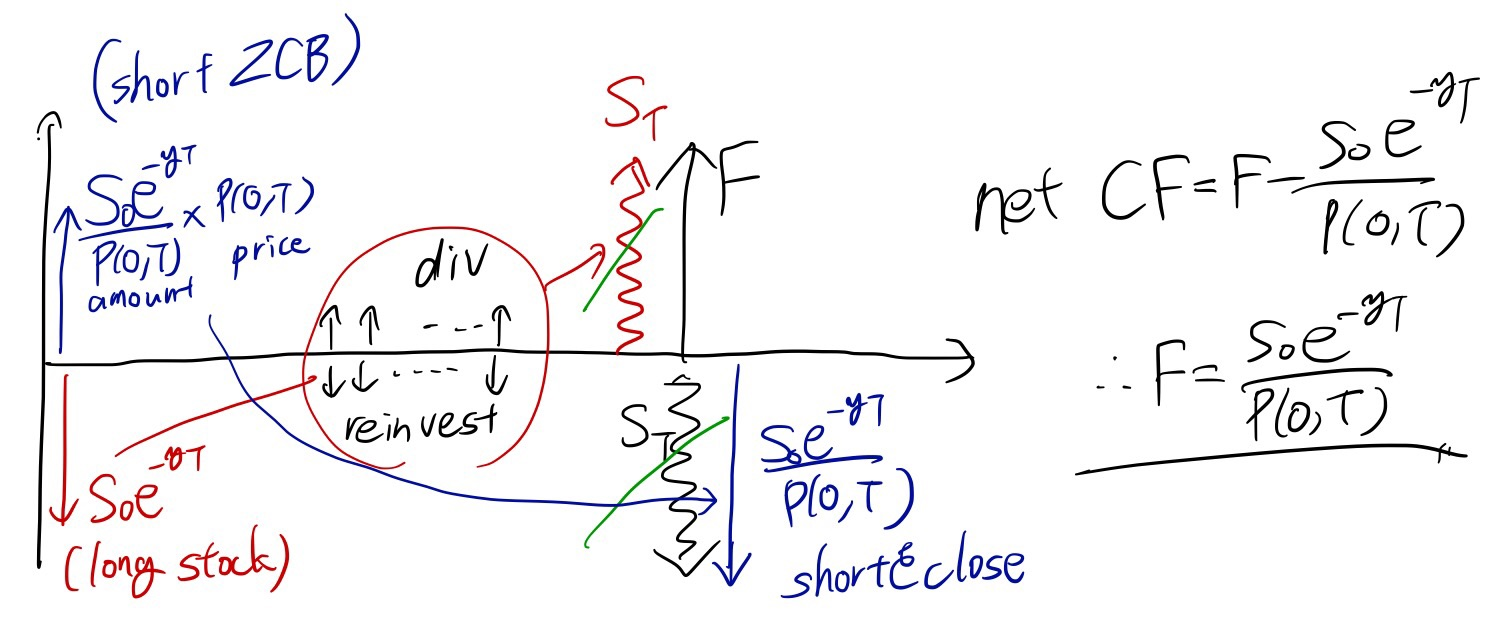
\includegraphics[width=10cm]{fig/1_2_02.JPG}
  \end{center}
\end{figure}

イメージ:
\begin{align}
  \mbox{P.V}(\mbox{receive} \, S_T \,\mbox{at} \, T)
  =F\times P(0,T)=\df{S_0}{P(0,T)}\times P(0,T)=S_0
\end{align}

randomなcash flowのP.V.を計算するときは,Forward Priceを求めて,
$P(0,T)$を乗じてやればよい(ただし市場がliquid,replicatableなときのみ)

$\Rightarrow$ 後にrisk-nuetralの下で計算すればわざわざreplicationを考える必要がなくなる


\subsubsection{Mark to Market of a fwd contract}
* P.V.(at $t=0$)\{fwd contract\}は0だが,時間が進むにつれて,
P.V.は変化する.

Suppose we entered the fwd contract to receive $X_T$
in exchange for a fixed amount of cash $F_0$
($F_0$ : fwd price at $t=0$). P.V.($t=0$)$=0$ \\
at time $t\in(0,T)$, suppose fwd price is given by $F_t$.
We want to know P.V.($t>0$).\\
Ans.:
\begin{align}
  \mbox{P.V.}(t)=P(t,T)(F_t-F_0)
\end{align}
\begin{prf}
  enter the new fwd contract at $t=t$
  (pays $X_T$ and receives $F_t$ at $t=T$) \\
  * $F_t$の$t$は「時刻$t$にcontractにenterした」という意味.

  (abbr.)
  \begin{align}
    \mbox{P.V.}(\mbox{at}\, t)
    \{\mbox{new + original fwd contracts}\}
    &=P(t,T)(F_t-F_0) \notag \\
    &=0+\mbox{P.V.}(\mbox{at}\, t)\{\mbox{original}\}
  \end{align}
\end{prf}

\subsubsection{Put-Call Parity}
\begin{definition}{(Call Option and Put Option)}
  A call (respectively, put) option on a certain index $X$
  with expiry $T$ and strike $K$ is the binomial?? contract
  to pay the holder of the option the cash amount equal to
  $\max(X_T-K,0)$, (resp, $\max(K-X_T,0)$)
\end{definition}

Let $C$ (resp, $P$) be the call (resp, put) option orice
(at $t=0$). We have the following put-call parity:
\begin{align}
  C-P=P(0,T)(F_X-K)
\end{align}
- $F_X$ : the fwd price of $X$ with mat. $T$
(時刻$t=X$ではなく,underlying asset $X$ をもとにした
fwd price at $t=0$)

\begin{prf}
  cash flow at $T$:
  \begin{align}
    \max(X_T,K,0)-\max(K-X_T,0)=X_T-K \\
  \end{align}
  Present value of above is given by:
  \begin{align}
    C-P=P(0,T)(F_X-K)
  \end{align}
\end{prf}

motivation:
\begin{itemize}
  \item liquidityの問題
  \item call, putの一方が求まれば,もう一方をすぐに求められる
  \item PDEの計算はputの方が簡単(because of boundary condition)
\end{itemize}



\subsection{Forward Rate Agreement and Interest Rate Swap}
*金利スワップはnot tradable

\subsubsection{Simple Rate and Day-Count Convention}
Suppose $T_i$ specifies the date $D_i=D(d_i, m_i, y_i)$
\begin{enumerate}
  \item{Actual/365}
  \begin{align}
    \delta(T_0, T_1)=\df{D_1-D_0}{365}
  \end{align}
  \item{Actual/360}
  \begin{align}
    \delta(T_0, T_1)=\df{D_1-D_0}{360}
  \end{align}
  \item{30/360}
  \begin{align}
    \delta(T_0, T_1)
    =\df{\max(30-d_0,0)+\min(d_1,30)+360(y_1-y_0)
    +30(m_1-m_0-1)}{360}
  \end{align}
  \item{actual/actual} considering leap year? 365 or 366
\end{enumerate}

\begin{definition}{(Simple Rate)}
  A (risk-free) simple rate (not compound) $L(T_{i-1},T_i)$
  with day-count $\delta(T_{i-1},T_i)$ is the interest rate with
  accrual convention defined in such a way that, when one invest
  $N$ amount of cash at $T_{i-1}$, then he receives
  $N(1+\delta_i L(T_{i-1},T_i))$ at time $T_i$.
  $L(T_{i-1},T_i)$ is the zero coupon rate at $T_{i-1}$
  for $[T_{i-1},T_i]$ with corresponding day-count convention.
\end{definition}
*accrual: ??

\subsubsection{Forward Rate Agreement (FRA)}
\begin{definition}{Forward Rate Agreement}
  A FRA is a binding(義務の) contract with the two parties
  (lender and borrower) agreeing to let a certain fixed rate $K$
  act on a prefixed notional amount $N$, over a future period
  $[T_M, T_N]$.
\end{definition}
*notional: 想定される?

\begin{definition}{Forward Rate}
  A forward rate $F$ for the period $[T_M,T_N]$ with day-count
  $\delta=\delta(T_M,T_N)$ is the fixed rate $K$ with the some
  day-count convention that makes the present value of the FRA zero.
\end{definition}

off course,
\begin{align}
  F=L(T_M, T_N) \quad (\mbox{at} \, T_M)
\end{align}
*$L$ : simple rate

\begin{lem}
  Let $\delta=\delta (T_M,T_N)$. Then the forward rate $F$
  at $t=0$ fot the period $[T_M,T_N]$ is given by
  \begin{align}
    F=\df{1}{\delta}\left(\df{P(0,T_M)}{P(0,T_N)}-1\right)
  \end{align}
  (*asm: liquid, no-arbitrage)

  \begin{prf}{replication strategy}
    \begin{itemize}
      \item Enter the FRA of rate $F$ to borrow
      unit amount of cash for $[T_M,T_N]$
      \item Sell one ZCB with mat. $T_N$ (short)
      \item Buy ZCB with mat. $T_N$ with principal amount
      $\df{P(0,T_M)}{P(0,T_N)}$
      \item At $T_M$, borrow unit amount of cash through FRA
      and use it to return ZCB
      \item At $T_N$, receive the principal $\df{P(0,T_M)}{P(0,T_N)}$,
      and pays $(1+\delta F)$
    \end{itemize}
    
    Net cash flow at $T_N$:
    $\left(\df{P(0,T_M)}{P(0,T_N)}\right)-(1+\delta F)$ \\
    If we require no-arbitrage, 
    \begin{align}
      \left(\df{P(0,T_M)}{P(0,T_N)}\right)-(1+\delta F)=0
      \quad \Rightarrow \quad
      F=\df{1}{\delta}\left(\df{P(0,T_M)}{P(0,T_N)}-1\right)
    \end{align}
  \end{prf}
\end{lem}

\begin{figure}[H] %HはHereを意味する
  \begin{center}
    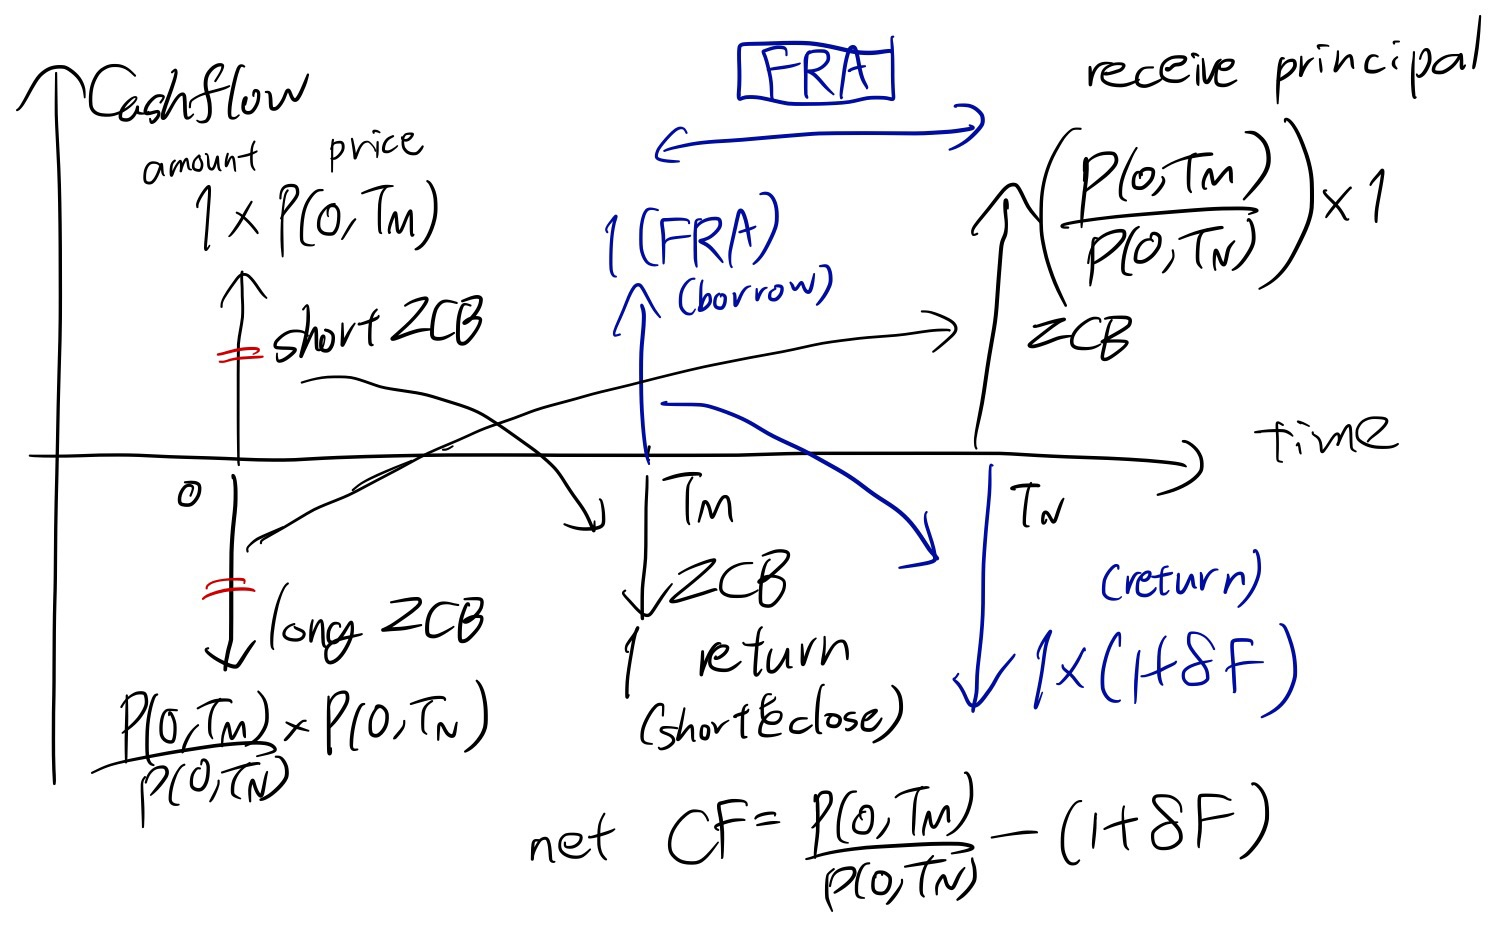
\includegraphics[width=10cm]{fig/1_3_01.JPG}
  \end{center}
\end{figure}


We write the above $F$ as
\begin{align}
  F(0,T_M,T_N)=\df{1}{\delta}\left(\df{P(0,T_M)}{P(0,T_N)}-1\right)
\end{align}
In general. at $t<T_M$,
\begin{align}
  F(t,T_M,T_N)=\df{1}{\delta}\left(\df{P(t,T_M)}{P(t,T_N)}-1\right)
\end{align}
$t\uparrow T_M$:
\begin{align}
  F(T_M,T_M,T_N)=\df{1}{\delta}\left(\df{1}{P(T_M,T_N)}-1\right)
  =L(T_M,T_N)
\end{align}

($\because$)
\begin{align}
  1=P(T_M,T_N)\{1+\delta L(T_M,T_N)\}
\end{align}
at $T_M$ invest 1, at $T_N$ return $1+\delta L(T_M,T_N)$ \\
(otherwise there exist arbitrage opportunities.) \\
(abbr.)

\begin{ex}
  Q) P.V.(at $0$) \{receive $1+\delta L(T_M,T_N)$\} ?
  $\rightarrow$ A) P.V.=0 \\
  ($\because$)
  Suppose that we are at $t=T_M$, $L(T_M,T_N)$ ... known 
  \begin{align}
    \mbox{P.V.}(\mbox{at} \, T_M)=-1+P(T_M,T_N)(1+\delta L(T_M,T_N))=0
  \end{align}
  将来のある時点($t=T_M$)でP.V.$=0$なら,さかのぼった
  $t=0$でも当然P.V.$=0$
  \begin{align}
    P.V.(\mbox{at} \, 0)\{\mbox{receive}\,
    1+\delta F(0,T_M,T_N) \, \mbox{at} \, T_N\}
    &= P.V.(\mbox{at} \, 0) \{\mbox{receive} \,
    1+\delta L(T_M,T_N)\} \\
    ( \therefore ) \quad
    P(0,T_N)F(0,T_M,T_N)&=P.V.(\mbox{at} \, 0)
    \{ \mbox{receive} \, L(T_M,T_N)  \}
  \end{align}
\end{ex}


\subsubsection{Fixed vs Floating Interest Swap}
Fix a time partition $0=T_0<T_1<...<T_M$

\begin{definition}{(Spot-start Swap)}
  A spot-start swap with maturity $T_M$ and notional amount
  $N$ is the contract in which one party (receiver)
  receives cash amount $NK\Delta_i$ ($K$ fixed)
  and pays the stochastic amount
  $NL(T_{i-1},T_i)\delta_i$ at every $T_i, \, i=\{1,2,...,M\}$.
  The other party (payer) has the opposit cash flow. Here,
  \begin{align}
    \begin{cases}
      \Delta_i &= \Delta(T_{i-1},T_i) \quad \mbox{(fixed)}\\
      \delta_i &= \delta(T_{i-1},T_i) \quad \mbox{(floating)}
    \end{cases}
  \end{align}
  are the day counts fot a fixed and floating payments, respectively.
\end{definition}

\begin{figure}[H] %HはHereを意味する
  \begin{center}
    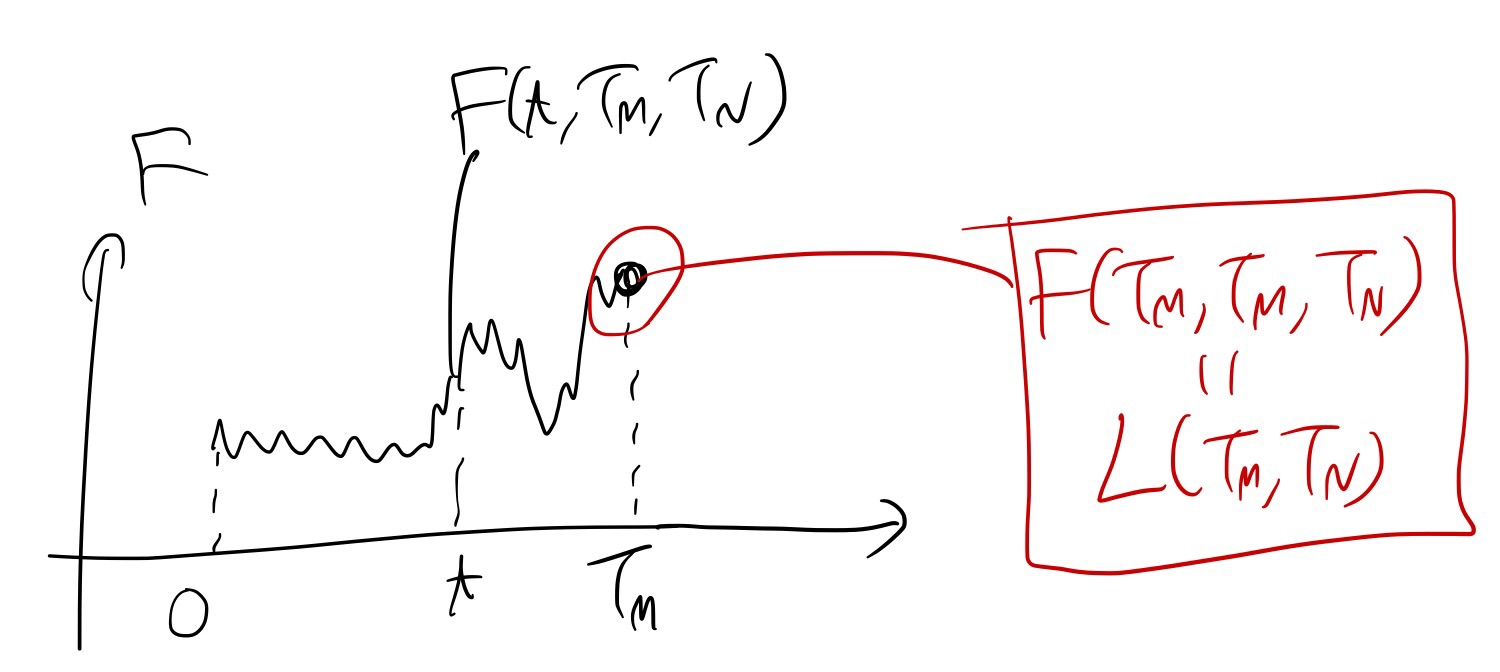
\includegraphics[width=10cm]{fig/1_3_02.JPG}
  \end{center}
\end{figure}


\begin{definition}{(Swap Rate)}
  The (spot) swap rate for the maturity $T_M$ is the fixed rate $K$
  that makes the present value of the swap zero.
\end{definition}

P.V. of the swap rate:
\begin{align}
  PV_{fix}&=NK\sum_{i=1}^M P(0,T_i)\Delta_i \\
  PV_{float}&=N\sum_{i=1}^M P(0,T_i)F(0,T_{i-1},T_i)\delta_i
  =N\sum_{i=1}^M P(0,T_i)
  \left(\df{P(0,T_{i-1})}{P(0,T_i)}-1\right) \notag \\
  &=N\sum_{i=1}^M (P(0,T_i)-P(0,T_i))
  =N(1-P(0,T_M))
\end{align}

Swap rate $K$:
\begin{align}
  K=\df{1-P(0,T_M)}{\sum_{i=1}^M P(0,T_i)\Delta_i}
  :=S(0;T_0,T_M)
\end{align}

* Economic meaning of swap rate:
\begin{align}
  S(0;T_0,T_M)
  =\df{\sum_{i=1}^M P(0,T_i)F(0,T_{i-1},T_i)\delta_i}
  {\sum_{i=1}^M \Delta_i P(0,T_i)}
\end{align}
Let us approximate as
\begin{align}
  P(0,T_i)\approx 1, \, \delta_i\approx\Delta_i
  \quad \mbox{for all} \, i \\
  \Rightarrow
  S(0;T_0,T_M)\approx\df{\sum_{i=1}^M F(0,T_{i-1},T_i)}{M} 
\end{align}
...average of fwd rates!

\begin{definition}{(Forward Swap)}
  A forward swap is the swap which starts at some future time.
  Fixed rate (fixed at $t=0$) which make the P.V. of the swap
  is called the forward swap rate.
\end{definition}

\begin{ex}
  A forward swap for the period $[T_M,T_N]$ \\
  $\Rightarrow$ cash flow exchanges
  at $T_i, \, i=\{M+1, ..., N\} $ \\
  $NK\Delta_i \, \leftrightarrow \, NL(T_{i-1},T_i)\delta_i$

  Let fixed rate be $K$, notional $=1$
  \begin{align}
    PV_{fix}&=NK\sum_{i=M+1}^N P(0,T_i)\Delta_i \\
    PV_{float}&=N\sum_{i=M+1}^N P(0,T_i)F(0,T_{i-1},T_i)
    \delta_i = P(0,T_M)-P(0,T_N)
  \end{align}
  Fwd Swap Rate:
  \begin{align}
    S(0;T_M,T_N)
    =\df{P(0,T_M)-P(0,T_N)}{\sum_{i=M+1}^N P(0,T_i)\Delta_i}
  \end{align}
\end{ex}


\subsubsection{Relation to the fixed coupon bond}
Consider the spot-start swap for $[T_0=0, T_N]$ (notional$=0$)
\begin{align}
  PV_{float}=\sum_{i=1}^N \delta_i P(0,T_i)F(0,T_{i-1},T_i)
  =1-P(0,T_N)
\end{align}
(abbr.)


Bond-Swap, Fixed vs Floating swap, 
???

defined $i(t)$ : index, $i\in\{0,...,N\} $
s.t. $t\in[T_i,T_{i+1}) \quad T_{i(t)}\leq t < T_{i(t)+1}$

\underline{current time $t$}
\begin{align}
  &\mbox{P.V.(floating leg?+ final principal)} \notag \\
  =&P(t,T_{i(t)+1})\delta_{i(t)+1}L(T_{i(t)},T_{i(t)+1})
  +\sum_{j=i(t)+2}^N P(t,T_j)\delta_j F(t,T_{j-1},T_j)
  +P(t,T_N) \notag \\
  =&P(t,T_{i(t)+1})\delta_{i(t)+1}L(T_{i(t)},T_{i(t)+1})
  +\sum_{j=i(t)+2}^N P(t,T_j)(1+\delta_{i(t)+1}L(T_i,T_{i+1}))
  +P(t,T_N) \notag \\
  =&P(t,T_{i(t)+1})(1+\delta_{i(t)+1}L(T_i,T_{i+1}))
  \approx 1
\end{align}

Thus, floating leg + final principal $\approx$ IR-RISK $0$

IR-Swap Risk $\approx$ fixed leg + final principal payment \\
$\Leftrightarrow$ fixed coupon Bond


\subsubsection{Yield Curve Construction (Simplified...)}
\begin{asm}
  There are market quotes of spot-starting swaps with swap rate
  $\{S_n\}_{n=1}^N$ with corresponding maturities $\{T_n\}_{n=1}^N$
  \begin{align}
    S_n:S(0;T_0,T_n), \quad T_0=0
  \end{align}
\end{asm}


\begin{ex}
  3 month. $0=T_0<T_1<...<T_N$
\end{ex}
We want to get $\{P(0,T_n)\}_{n=1}^N$ which are consistent with
the swap quotes.

1) Determin $P(0,T_1)$
\begin{align}
  S_1 \Delta_1 P(0,T_1)=P(0,T_0)-P(0,T_1) \\
  S_1 = \df{1-P(0,T_1)}{\Delta_1 P(0,T_1)} \\
  P(0,T_1)=\df{P(0,T_0)}{1+\Delta_1 S_1}=\df{1}{1+\Delta_1 S_1}
\end{align}

2) Suppose we have obtained $\{P(0,T_n)\}_{n=1}^{m-1}$.
Consider $T_m$-maurity swap:
\begin{align}
  S_m \Delta_m P(0,T_m)+S_m \sum_{n=1}^{m-1} \Delta_n P(0,T_n)
  =1-P(0,T_m) \\
  \Rightarrow \, (*) \quad
  P(0,T_m)=\df{1-S_m\{\sum_{n=1}^{m-1}\Delta_n P(0,T_n)\}}
  {1+\Delta_m S_m}
\end{align}
using
\begin{align}
  (*) \quad S_m=S(0;T_0,T_m)
  =\df{\sum_{n=1}^{m}\Delta_n P(0,T_n)}{1-P(0,T_m)}
\end{align}

yield curve ... to be interpolated


\subsubsection{Market-to-Market fo a forward swap}
Suppose has swap starting $T_M$ with maturity $T_N$
as a receiver (long bond party) with the fixed rate $X$,
notional $L$.
Suppose the current $(t=0)$ market quotes is given by
$S(0,T_M,T_N)$.

\begin{align}
  PV(t=0) &= LX\sum_{n=M+1}^N \Delta_n P(0,T_n)
  -L\sum_{n=M+1}^{N}P(0,T_n)\delta_n P(0,T_n)F(0,T_{n-1},T_n)
  \notag\\
  &=L\sum_{n=M+1}^{N}\Delta_n P(0,T_n)(X-S(0,T_M,T_N))
\end{align}
bondのreceiverは金利が下がったら嬉しい

\subsubsection{Approximation of a fwd swap rate}
\begin{align}
  S(0,T_M,T_N)&=\df{P(0,T_M)-P(0,T_N)}
  {\sum_{i=M+1}^N \Delta_i P(0,T_i)}
  =\df{\sum_{i=M+1}^N \delta_i F(0,T_{i-1},T_i)P(0,T_i)}
  {\sum_{i=M+1}^N \Delta_i P(0,T_i)} \notag \\
  &\approx \df{1}{N-M} \sum_{i=M+1}^N F(0,T_{i-1},F_i)
  \quad (as \, \delta_i\approx\Delta_i, \, P(0,T_i)=1)
\end{align}

$0<T_M<T_N$:
\begin{align}
  NS(0;T_0,T_N)\approx MS(0;T_0,T_M)+(N-M)S(0;T_M,T_N)
\end{align}
$NS(0;T_0,T_N)\approx$ \{$[T_0,T_N]$のfwd rateのsum\}

\begin{align}
  (\therefore) S(0;T_M,T_N) &\approx
  \df{NS(0;T_0,T_M)-MS(0;T_0,T_M)}{N-M} \notag \\
  &\approx \df{T_N}{T_N-T_M}S(0;T_0,T_N)
  -\df{T_M}{T_N-T_M}S(0;T_0,T_M)
\end{align}


\subsubsection{Deltas}
* market quotes (input) spot-swap rates $(S_n)_{n=1}^N$
$\Rightarrow$ $P(0,T)$ $\Rightarrow$ pricing...

Delas(PVO 1s)


P.V. of receive swap $[T_M, T_N]$.
Notional: $L$, fixed rate: $X$
\begin{align}
  P.V.(t=0)=L\sum_{i=M+1}^N\Delta_i P(0,T_i)(X-S(0;T_M,T_N))
\end{align}
Suppose the market change induces
\begin{align}
  S(0;T_M,T_N) \, \rightarrow \, S(0;T_M,T_N) + \delta S
\end{align}
then, change of the P.V. :
\begin{align}
  \delta P.V.=&L\sum_{i=M+1}^N\Delta_i(\delta P(0,T_i))
  (X-S(0;T_M,T_N)) \notag \\
  &+L\sum_{i=M+1}^N\Delta_i P(0,T_i)
  (-\delta S_M,N) + \mbox{higher order}
\end{align}

1st term order $\sim$ $1R^2$ \\
2nd term order $\sim$ $1R^1$ \\
$||\mbox{1st term}|| << ||\mbox{2nd term}||$

\begin{align}
  \delta P.V. \approx L\sum_{i=M+1}^N\Delta_i P(0,T_i)
  (-\delta S_M,N)
\end{align}
* $(-\delta S_M,N)$ : fwd swap rateの変化


\begin{align}
  S(0;T_M,T_N)&\approx\df{T_N}{T_N-T_M}S(0;T_0,T_N)
  -\df{T_M}{T_N-T_M}S(0;T_0,T_M) \\
  \delta S_{M,N}&\approx\df{T_N}{T_N-T_M}\delta S_N
  -\df{T_M}{T_N-T_M}\delta S_M
\end{align}

\begin{itemize}
  \item $\delta S_N$ : change of $S(0,T_0,T_N)$
  \item $\delta S_M$ : change of $S(0,T_0,T_M)$ 
\end{itemize}

\begin{align}
  &\delta P.V. (\mbox{fwd swap} \, (T_M,T_N)) \notag\\
  \approx& -L\sum_{i=M+1}^N\Delta_i P(0,T_i)
  \left\{\df{T_N}{T_N-T_M}\delta S_N
  -\df{T_M}{T_N-T_M}\delta S_M \right\} \notag \\
  \approx&-L(T_N-T_M)\times \df{1}{T_N-T_M}
  (T_N\delta S_N-T_M\delta S_M) \quad
  (\mbox{approx.}\, P(0,T_i)\approx 1 ) \notag \\
  =&-L(T_N\delta S_N-T_M \delta S_M)
\end{align}
(* day-count conventionのズレは無視)

\begin{itemize}
  \item spot-start swap
  \item maturity $T_N$
  \item Notional $L$
\end{itemize}
receiver:
\begin{align}
  \delta P.V.=-L\times T_N\times\delta S_N
\end{align}


\newpage
\section{Binomial Model}
多期間モデルは連続モデルへの直観を与える.
PDEの数値計算との関連もあり.

\subsection{One-Period Binomial Model}
\subsubsection{Model Description}

There are two points in time $t=0,T$.
Two tradable assets:
\begin{itemize}
  \item Bond (risk-free asset)
  \begin{align}
    B_0&=1 \\
    B_T&=e^{rT}
  \end{align}
  (deterministic) \\
  $r$: zero rate for $[0,T]$ at $T=0$
  \item Stock (risky asset)
  \begin{align}
    S_0&=s \, (>0) \\ 
    S_T&=
    \begin{cases}
      su \quad \mbox{with prob.} \, P_u \\
      sd \quad \mbox{with prob.} \, P_d
    \end{cases} \\
    &P_u>0, \, P_d>0, \, P_u+P_d=1, \, 0<d<u
  \end{align}
  We write for simplicity:
  \begin{align}
    S_T&=sZ \\
    Z&=
    \begin{cases}
      u \quad \mbox{with prob.} \, P_u \\
      d \quad \mbox{with prob.} \, P_d
    \end{cases}
  \end{align}
  under emprical measure $\mathbb{P}$, 
  $\mathbb{P}(\{up\})=P_u, \,
  \mathbb{P}(\{down\})=P_d$
\end{itemize}

Portfolio : $h(x,y) \quad x,y\in\mathbb{R}$
\begin{itemize}
  \item $x$: number of position for the bond
  \item $y$: number of position for the stock
\end{itemize}

the value process of the portfolio $h$:
\begin{align}
  V_t^h&=xB_t+yS_t \quad \mbox{in general} \\
  V_0^h&=x+ys \\
  V_T^h&=xe^{rT}+ysZ
\end{align}

\begin{definition}
  An arbitrage portfikui us a portfolio with the properties:
  \begin{align}
    V_0^h=0, \, P(V_T^h\geq 0)=1, \, P(V_T^h>0)>0
  \end{align}
  * no-arbitrage $\Rightarrow$ existence of risk neutral measure
  (we'll see later)
\end{definition}

\begin{prop}\label{prop_af}
  The one-period binomial model is arbitrage free
  iff (=if and only if) the following condition holds:
  \begin{align}\label{cond_af}
    0 < d < e^{rT} <u
  \end{align}

  \begin{prf}{proof of above prop.} 
    
    \begin{itemize}
      \item (necessarity = only if):
      Suppose \ref{cond_af} does not hold.
      \begin{enumerate}
        \item $e^{rT}\leq d < u$
        \begin{enumerate}
          \item Sell the Bond $s$ units
          \item Buy one unit of the stock
        \end{enumerate}
        $h(x,y)=(-s,1)$, net cf $=0$ at $t=0$.
        Then,
        \begin{align}
          V_T^h=-se^{rT}+sZ=s(-e^{rT}+Z)
        \end{align}
        It's clear that $V_T \geq 0$, $P(V_T\geq 0)=1$.
        \begin{align}
          P(V_T^h>0)=P(Z=u)=P_u>0
        \end{align}
        Therefore, arbitrage.

        \item $d < u \leq e^{rT}$ \\
        各自考えよ
      \end{enumerate}

      \item (sufficiency = if):
      Suppose \ref{cond_af} holds. \\
      Assume $V_0^h=0$ then $x+ys=0 \, \Rightarrow \, ys=-x$.
      \begin{align}
        &V_T^h =xe^{rT}+ysZ=x(e^{rT}-Z) \\
        &P(V_T^h\geq 0) < 1
      \end{align}
      Therefore, no-arbitrage.

    \end{itemize}
  \end{prf}

\end{prop}

\subsubsection{Risk-neutral Probability Measure}
Suppose $d<e^{rT}<u$ holds, \\
$\Rightarrow$ one can find $q_u, \, q_d \, >0$ s.t.

\begin{align}
  \begin{cases}
    q_u+q_d=1 \\
    q_d u+q_d d=e^{rT}
  \end{cases} \\
  \Rightarrow
  \begin{cases}
    q_u=\df{e^{rT}-d}{u-d} \quad (>0) \\
    q_d=\df{u-e^{rT}}{u-d} \quad (>0)
  \end{cases}
\end{align}
We define a new (and not emprical) probability measure
$\mathbb{Q}$ such that
\begin{align}
  \mathbb{Q}(Z=u)&=q_u \\
  \mathbb{Q}(Z=d)&=q_d
\end{align}
It's interesting to observe that
\begin{align}
  e^{-rT}\mathrm{E}^{\mathbb{Q}}[S_T]
  &=e^{-rT}(q_u\times su+q_d\times sd) \notag \\
  &=se^{-rT}(q_u u+q_d d)=s\,(=S_0)
\end{align}

In general,
\begin{align}
  \{\ e^{-rT}S_t \}_{t=0,T} \quad ... \, \mathbb{Q}
  \mbox{-martingale}
\end{align}

\begin{definition}{(Risk-neutral Measure)}
  The probability measure $\mathbb{Q}$ with associated
  probability $(q_u, q_d)$ satisfying the condition
  eq\eqref{cond_af} is called the risk-neutral measure.
\end{definition}

\begin{prop}
  The one-period binomial model just explained is arbitrage
  free iff there exists a risk-neutral measure
  $\mathbb{Q}$ ($q_u>0,\, q_d>0)$
\end{prop}

\begin{prf}
  arbitrage free $\Leftrightarrow$ $d<e^{rT}<u$
  ($\because$ Prop. \ref{prop_af}) \\
  \begin{align}
    &\mathbb{Q}=(q_u,q_d) \\
    &q_u=\df{e^{rT}-d}{u-d} , \quad
    q_d=\df{u-e^{rT}}{u-d} \\
    &q_u+q_d=1
  \end{align}

  If such $\mathbb{Q}$ exists, then
  \begin{align}
    & \exists q_u,q_d \, >0 \quad \mbox{s.t.}
    \begin{cases}
      q_u+q_d=1 \\
      q_u u + q_d d =e^{rT}
    \end{cases} \\
    \Rightarrow & \, d<e^{rT}<u
  \end{align}
\end{prf}

\subsubsection{Risk-neutral Pricing}
\begin{definition}{(Contingent Claim)}
  A contingent claim is any random cash flow $X_T$ at $T$
  of the form $X_T=\Phi(S_T)$ with some function $\Phi$.

  \begin{ex}{(call option with strike $K$)}
    \begin{align}
      \Phi(S_T)=\max(S_T-K,0)=(S_T-K)^{+}
    \end{align}
  \end{ex}
\end{definition}

\begin{definition}{(Replicable / Complete)}
  A given contingent claim $X$ is said to be replicatable
  (or perfectly hedgeable) if there exists a portfolio $h$
  such that $V_T^h=X_T$ with probability $1$ (under $\mathbb{P}$).
  In this case, we call $h$ a replicating portfolio of $X$.
  If all contingent claim are replicable, we say
  the market is complete. Otherwise the market is incomplete.
\end{definition}

\begin{prop}
  Suppose that a contingent claim $X$ is replicable by
  portfolio $h$. Then, any price at $t=0$ of the claim $X$
  other than $V_0^h$ will lead to an arbitrage opportunity.
\end{prop}

\begin{prf}
  Suppose $h$ is given by $h=(x,y)$. Suppose $V_0^h\neq X_0$.
  \begin{enumerate}
    \item $V_0^h<X_0$
    \begin{itemize}
      \item Short the contingent claim $X$ (one gets $X_0$)
      \item Construct a portfolio $h(x,y)$ : $V_0^h=x+sy$
      \item Buy $(X_0-V_0^h)$ units of bond 
    \end{itemize}
    portfolio $h'=(x+X_0-V_0^h, y)$ + short position of $X$ \\
    net cash flow at $T$:
    \begin{align}
      V_T^{h'}-X_T=(X_0-V_0^h)e^{rT}+V_T^h -X_T
      =(X_0-V_0^h)e^{rT} > 0
    \end{align}  
    $\rightarrow$ arbitrage.
    \item $V_0^h>X_0$
    \begin{itemize}
      \item Buy the contingent claim $X$
      \item Short the replicating portfolio $h(x,y)$
      : $V_0^h=x+sy$
      \item Buy $(V_0^h-X_0)$ units of bond 
    \end{itemize}
    portfolio $h''=(V_0^h-X_0-x, -y)$ + long position of $X$ \\
    net cash flow at $T$:
    \begin{align}
      V_T^{h''}+X_T=(V_0^h-X_0)e^{rT}-V_T^h +X_T
      =(V_0^h-X_0)e^{rT} > 0
    \end{align}  
    $\rightarrow$ arbitrage.
  \end{enumerate}
\end{prf}


\begin{prop}
  The binomial model is complete.
\end{prop}

\begin{prf}
  Consider a general contingent claim $X$
  whose payoff at $T$ is $\Phi(S_T)$.
  $\Phi : \mathbb{R} \to \mathbb{R}$ function.
  \begin{ex}
    Call option $\Phi(S_T)=\max(S_T-K,0), \quad K\in\mathbb{R}$\\
    It suffices to construct a strategy $h=(x,y)$ s.t.
  \end{ex}
\end{prf}



\subsection{The Multi-Period Binomial Model}
\subsubsection{Model Description}
$0=t_0<t_1<...<t_N=T$

\newpage
\section{I\^{t}o Formula and Option Valuation}
\subsection{Probability Space}



\end{document}
